\chapter{INTRODUCTION}
\label{INTRODUCTION}
%Wireless networks utilize radio waves instead of wires to carry information, hence seamless coverage and mobility are achievable in wireless connections.
Wireless networks have experienced unprecedented growth in the past few decades and will going on evolving in the future.
Due to the propagation characteristics and regulations, only a small portion of electromagnetic spectrum which spans from 8.3 kHz to 3000 GHz is suitable for commercial application.
These spectrum is divided into bands (also referred as channels) and allocated to different services.
%In the following, we introduce how is the spectrum accessed by different services.
%
As one kind of limited and precious resource, radio spectrum is strictly regulated by the national administration.
The channels are assigned or leased by governments to different operators and entities.
In most cases, the operators pay high price for the commercial usage of certain spectrum, and the usage is exclusive for them~\cite{Spectrum_Management07}.
This spectrum management policy rules out the unlicensed users to use the spectrum, thus strictly protects the interest of the spectrum licensees.
This spectrum access module is referred \textit{exclusive use model}~\cite{zhao_survey_DSA_2007}, and is the mainstream of spectrum access worldwide, and many existing wireless applications work on the licensed spectrum.
For instance, the second-generation (2G) wireless cellular network GSM (global system for mobile communications) in Europe works with GSM-900 band (from 890 MHz to 960 MHz) and GSM-1800 (1710 MHz to 1880 MHz), and the third-generation (3G) wireless cellular network works from 1.8 GHz to 2.4 GHz~\cite{wireless_communicatioins2001}.
The excludability of licensed spectrum can also be open to other user with conditions.
The spectrum licences either sell and trade the licensed spectrum, or dynamically use the spectrum within a certain region according to different traffic patterns~\cite{dsa_traffic_2000}.
Open spectrum access~\cite{osa_Noam_1995} is proposed in 1995 for full openness of entry, which allows access to spectrum through access fees which are determined by demand and supply.
It is claimed that open spectrum access brings in benefits, as for spectrum licensees, the fixed costs on securing the licensed spectrum can be converted into marginal costs, and for the market, the incentives for collusive pricing can be eliminated.
But as the \textit{openness} here is fully controlled by the licensees, this spectrum usage is still exclusive .

%
In contrary to exclusive use model, certain spectrum are assigned for open sharing for peer users, the representative example is the unlicensed industrial, scientific, and medical (ISM) radio band, which supports versatile wireless applications and a prosperous industry, \ie WiFi.
Many spectrum sharing strategies are proposed to cope with the technical challenges~\cite{Ko_DistributedCA}.

\section{Hierarchical Spectrum Access Model}
\label{hierarchical}
The proliferation of wireless network constantly arises urgent demand on bandwidth and throughput since the first generation of telecommunication in 1980s, which accordingly encourages the efficient use and reuse of the electromagnetic spectrum.
The next generation of telecommunication technology 5G, which is reported to come true in 2020, requires a leap forward of spectrum efficiency~\cite{5G_2014}.
The resorted applications under the label of 5G~\cite{5directions5G_2014}, \ie machine to machine communication, internet of things, etc, requires high speed and lower investment cost, but this is changeling as the achieved capacity approaches Shannon capacity, and most spectrum are licensed.
Meanwhile, the actual spectrum usage measurement conducted by FCC tells that at many locations or time, the licensed spectrum is idle~\cite{FCC_spectrumEfficiency_2002}, and there exists a large number of spectrum bands which have considerable dormant time intervals ~\cite{Akyildiz06survey}.


To seek more opportunities from spectrum, it is natural to consider opening the licensed spectrum to unlicensed users, if the interference perceived by licensed users are restricted.
We adopt the terms proposed in~\cite{zhao_survey_DSA_2007}, and call this spectrum usage policy as \textit{hierarchical access model}, where licensed users are called primary users, and unlicensed users are named as secondary users.
Hierarchical access model gives a promising solution to the reclamation of new electromagnetic spectrum and the improvement of spectrum efficiency.

In respect of the relation between primary and secondary users, there are two spectrum sharing paradigms.
\begin{itemize}
\item The first approach is \textit{spectrum underlay}, where the interference generated by secondary users on the primary receivers should be under a threshold. 
This kind of spectrum sharing restricts the secondary users' transmission power, but is able to achieve high data rate in short range.
Spectrum underlay is mainly conducted with a centralized controller, which has global knowledge of primary users' location, the attenuation between all secondary transmitters and all primary receivers.
Then the centralized controller calculates the maximal permitted transmission power with certain optimization solutions in a situation where secondary users pose the maximal thread to primary users' operation, where all the secondary users work one the same licensed spectrum.
%secondary users at certain locations are restricted to operate on a few certain spectrum bands and with limited transmit power~\cite{whitefi09}.
%Given the attenuation between all secondary transmitters and all primary receivers and their locations, when the interference threshold is known, the maximal permitted transmission power levels of secondary transmitters can be obtained with linear programming.
In spectrum underlay paradigm, secondary users do not need to sense the existence of primary users.

\item The other approach is \textit{spectrum overlay}, where secondary transmitters are only allowed to transmit when the primary users are detected as being idle.
In this paradigm, secondary users should monitor the spectrum of interest preactively to detect primary users' appearance.
The detection metrics include received primary users' signal power, spectral correlation or beacons~\cite{crnsensing_09}.
Spectrum sensing requires sophisticated technologies when primary users' signal is weak, and can be improved by learning technologies or cooperation among multiple secondary users~\cite{coorperativeSensing_Akyildiz11}.
When spectrum sensing accuracy can be guaranteed above certain threshold, transmission power restrictions can be removed from  secondary users.
\end{itemize}

%


Spectrum administration bodies FCC of U.S.~\cite{FCC_2010_sedond_memorandumm} and Electronic Communications Committee (ECC) in Europe~\cite{ecc159} encourage to adopt both spectrum sensing and location based method.
%Secondary users' operation is restricted on certain spectrum bands and transmit power should be below certain threshold according  to their locations, and spectrum sensing ability is also required.


%\subsection{Spectrum Access Etiquette in Cognitive Radio Network}
%
%%CR users utilize the unused licensed spectrum opportunistically and meanwhile avoid interfering licensed users.
%%This new spectrum usage paradigm imposes great challenge to the CR users, including how to detect the licensed users and afterwards decide on the suitable spectrum and on which interact with other CR users.
%
%%Before the emerging of cognitive radio technology, spectrum is allocated in a fixed way, \ie certain chunk of spectrum is exclusively licensed to an certain entity by administration body.
%%The equipments which are given the license to utilize the spectrum is called licensed users, while the others which called unlicensed users are not allowed to work on the that part of spectrum.
%%This paradigm rigidly protects the benefit of licensed users, but it results in underutilization of spectrum.
%%Due to the drastic increase of mobile data applications there is an urgent demand on spectrum resources. 
%%Traditionally, frequency bands have been assigned exclusively to licensed bodies which can occupy the spectrum whenever there is information to be transmitted. 
%
%%This static spectrum utilization has been proven to be suitable for many systems and applications. 
%%However, as mobile networks have proliferated drastically over the last thirty years, this exclusive assignment has created a significant shortage of spectrum today. 
%
%Licensed users access their allocated spectrum band whenever there is information to be transmitted, in contrary, CR users are only allowed to access licensed spectrum after validating the channel is idle or the primary user is not to be affected if they operate on the licensed spectrum.
%In this thesis, licensed users are referred as primary users, and CR users are denoted as secondary users.
%
%The assessment of spectrum is a bone of contention for primary/secondary users and administration bodies.
%Spectrum sensing on secondary users is one common method to validate spectrum availability especially in research domain~\cite{crnsensing_09}.
%%Secondary users should monitor the spectrum of interest actively and autonomously to detect primary users' appearance.
%%Primary users can be detected by judging the primary users' signal power, spectral correlation or beacons.
%%Spectrum sensing requires sophisticated technologies when primary users' signal is weak.
%%Primary detection can be improved by learning technologies or cooperation among multiple secondary users~\cite{coorperativeSensing_Akyildiz11}.
%Another way to protect the primary users from being affected by secondary users' operation relies on location identification and certain operating rule set.
%Based on the global information of primary users' location and terrain information, centralized controller regulates that the secondary users at certain locations are restricted to operate on a few certain spectrum bands and with limited transmit power~\cite{whitefi09}.



%In contrast, CR users (forming cognitive radio networks, abbreviated as CRN) 
%This refers to the process of sensing a particular channel and verifying (with a previously specified probability of error) that it is not used by a primary user currently  [cite spectrum sensing].
%This form of spectrum sharing is also referred to as opportunistic spectrum access~\cite{Akyildiz06survey}.

%Such co-existence with primary users imposes great challenges for the CR users.
%On the first hand, CR users should be able to sense the channel to avoid interfering primary users.
%it is fairly easy to see that the sensing ability of secondary users plays an important role in the harmonious co-existence of primary and secondary users~\cite{09spectrumSensing_survey}.





\section{Cognitive Radio}
%\cite{spectrumSharingGames_interference_stackelberg_2009, spectrum_sharing_games_2010} spacial opportunistic allocation.


Throughout this thesis, we use \textit{cognitive radio networks} to compound the networks composed with secondary users which work in either spectrum underlay or spectrum overlay style.
There are two reasons, firstly, this name explicitly tells a distinctive property of the devices in the networks, their cognition to their environment, secondly, cognitive radio has become a synonym of the technology employed in the hierarchical spectrum access paradigm in academia and industry in the recent years.



%The dilemma that spectrum scarcity coexists with spectrum underutilization promotes cognitive radio (CR) as a promising technology to make full use of spectrum and accordingly solve the spectrum shortage problem.

The definition of cognitive radio evolves with the development of radio technology and regulations.
We choose two representative definitions to give a formal description of cognitive radio.
Cognitive radio is firstly proposed by Mitola III who defines the concept of CR in his dissertation~\cite{2000mitola_cognitive_radio} as follows:
%
\blockquote{... personal digital assistants (PDAs) and the related networks are sufficiently computationally intelligent about radio resources and related computer-to-computer communications to detect user communications needs as a function of use context, and to provide radio resources and wireless services most appropriate to those needs.
}

FCC (Federal Communications Commission in U.S.) describes CR~\cite{FCC_03-322} as,
\blockquote{
a radio that can change its transmitter parameters based on interaction with the environment in which it operates. $\ldots$
This interaction may involve active negotiations with other spectrum users and/or passive sensing and decision making (smart radio) within the radio. The majority of CRs will probably be SDRs~\footnote{software defined radio is a radio communication system which is able to receive any modulation across a large frequency spectrum, and transmit on desired spectrum band.}, but a CR does not necessarily use software, nor does it need to be field programmable.
}

In this thesis, we see cognitive radio as a device which is able to sense, detect, learn and monitor the surrounding radio frequency environment, or to access a certain database to retrieve primary users' information, so as to reconfigure its radio operating parameters (e.g. center frequency, bandwidth and transmit power) on the fly to avoid interfering primary users.
Cognitive radio may only practice one portion of the aforementioned functionalities according to actual situation.
Apparently, the cognitive radio users which conduct spectrum sensing are usually work with spectrum overlay paradigm, and the cognitive radio users which have means to get information of primary users are suitable to work with spectrum underlay paradigm.
Based on this definition, throughout this thesis the secondary users working with both spectrum underlay and overlay are named as cognitive radio users, besides, the cognitive radio network is deemed to be composed with cognitive radio users, whose acronym is CRN.



\subsection{Spectrum Management}
To adapt to dynamic spectrum environment and make use of the available licensed spectrum, cognitive radio users need to manage the available spectrum by conducting the following procedures sequentially, which include detecting the available spectrum with spectrum sensing, selecting the proper spectrum for communication, and sharing the spectrum with other secondary users.
These functions are incorporated into so called cognitive cycle as described in~\cite{Akyildiz09}.

To know which chunk of spectrum is available is the foundation of spectrum management.
In underlay spectrum usage scenario, CR users get to know the available spectrum by means of spectrum sensing.
In overlay spectrum usage scenario, secondary users can in principle access all the licensed spectrum.
In this procedure, quality of the available channels is determined with several parameters, \ie band width, operating frequency, path loss, wireless link errors, link layer delay, and the upper bound of interference on the primary user working on that channel, which decides the maximal permissible transmission power of secondary users.
Besides, the statistical behaviours of primary users is also an important factor.
%
After knowing the available spectrum, CR users select the most appropriate band according to their requirements on quality of service (QoS).
This procedure involves considering the statistical behaviours of the primary users so as to accessing the channel quality fairly.
%
Then secondary users are to make use of these selected channels, or in other words, to share the spectrum with other secondary users. 
As there may be multiple secondary users trying to use the same channel, spectrum sharing is important to coordinate the behaviour of secondary users to avoid deteriorating the performance of secondary users.
Spectrum sharing involves choosing proper channels to mitigate co-channel or adjacent interference, or adjusting transmission power to achieve promise between transmitter's and other secondary users' performance, or adopting a certain media access paradigm to use the spectrum fairly and efficiently.

%\todo[inline]{spectrum opportunity, detection, tracking, exploitation (whether to access, how to access, sharing),  tazhaosurveyDSA2007.}

%According to \cite{08crn_survey}, 	
%After assessing RF environment or geographic location, secondary users adjust their operational parameters such as frequency, modulation schemes and transmit power, in order to support QoS aware communications, this process is referred as spectrum decision and spectrum sharing~\cite{08crn_survey}.
%In this thesis, spectrum decision and sharing consist the major issue discussed in this thesis.

Some work in research community models the spectrum availability with stochastic or statistic model, which is helpful when deciding which channel to use.
\cite{Discrete-Time_Spectrum_Occupancy_Model_DySPAN_2011} proposes discrete Markov chain and adjusts duty circle models to describe the availability of licensed spectrum for GSM on 900/1800 MHz.
\cite{Wellens200910} models the channel holding time with geometric and log-normal distributions.
Statistics of previous sensing results is used to predict spectrum state in the future~\cite{spectrum-discovery-tmc08}.
Such models provide more complete information on the availability of the licensed channels.

The available licensed spectrum which spans a wide frequency band exhibits different characteristics~\cite{spectrum_decision_TMC11}.
Based on the requirements of interested communication, CR users need to identify the characteristics of the spectrum, which include channel quality (channel capacity, error rate, path loss, etc.)~\cite{spectrum_decision_TMC11}, channel switching delay~\cite{channel_switch_delay11}, and channel holding time, \ie the expected time duration that the primary users don't occupy the channel before any one occupies again.

\subsection{Spectrum Sharing}
How is licensed spectrum shared between primary and secondary users is introduced in Section~\ref{hierarchical}, spectrum sharing can also be classified by network architecture and spectrum allocation behaviour~\cite{Akyildiz09} respectively.
In this section, we introduce these classifications to vision spectrum sharing from different prospectives.
\subsubsection*{Classification Based on Architecture}
Based on architecture, spectrum sharing can be classified as centralized and distributed spectrum sharing.
As the name indicates, the centralized spectrum sharing relies on a centralized entity where the strategy to use the spectrum is decided. 

This pattern involves transmission overhead in collecting sensing result and distributing spectrum usage strategy.
There is considerable number of centralized approaches proposed for spectrum sharing in cognitive radio network, global optimality is reported as to different objectives, but centralized solution is not suitable in many real world situations.
First, central authority or controller is not available in many CRNs.
Second, Even the centralized decision maker exists, the centralized entity needs to collect spectrum availability sensed on all the secondary users in the network, then computes the spectrum usage strategy and distributes it.
A huge number of control messages are generated in this process, and it becomes worse when the update of channel availability is frequent due to primary users changing their states quickly.
%As to cognitive radio network, implementation of centralized algorithm faces more challenges.
%The central controller needs to know the network connectivity which is decided by the availability of licensed spectrum, or even the information of the later.
%Either the controller enquiring each secondary user for spectrum availability information, or the secondary users pushing to the controller introduces huge amount of overheads, especially when the primary users change their operation state frequently
%When the licensed users change their operation state frequently, centralized decision maker obtaining the updated sensing results from CR users imposes a great burden on the network.
Centralized scheme is suitable in certain scenarios, c, \eg when the primary users are TV stations and receivers which work on certain channels for hours of time, spectrum can be seen as constant. 
When the secondary users access the spectrum in underlay paradigm, they need to take care not to cause more interference than threshold on primary users.
In this case the channel usage, \ie working channel and transmission power, can be decided on the centralized controller.
%In this case, it is also possible that the centralized controller is only responsible to regulating the maximal transmission power to protect the licensed users from interference, but doesn't control secondary users' transmission strategy as they may belong to different business groups.

%Without infrastructure support, it is hard for CR user to get complete and up to date picture of the spectrum availability in the whole network.
%Thus distributed solutions are preferred in such varying radio environment.
%Distributed decision of one CR user should be carefully decided as one CR's behaviour affects neighbouring CR users which go on to prompt all the CR users in the network to act accordingly.

As to distributed spectrum sharing paradigm, secondary users need to autonomously decide their spectrum usage strategies, whereas they may be allowed to interact with other network entities in certain ways, \ie other secondary users and centralized database in IEEE 802.22 cellular network.
Distributed scheme requires message exchanges between secondary users during interaction.
Distributed decision of one CR user should be carefully decided as one CR's behaviour affects neighbouring CR users which go on to prompt all the CR users in the network to act accordingly.
In this thesis, the interaction between CR users will be discussed under game theoretical framework.

%because it is costly to retrieve necessary information from the network to the controller, which includes the spectrum information on each CR users and the network topology. Besides, when the solution is sent back to the CR users, the network state may have changed and be different from the time when the information is collected.

%This is due to the operation of primary users, which is usually not known by secondary users.
%The distinctive view on spectrum availability and varying radio environment make distributed solution a natural choice for CRN network.
% tendius text
\subsubsection*{Classification Based on Whether or Not to Cooperate}
Spectrum sharing can also be categorized into cooperative and non-cooperative spectrum sharing.
As to cooperative spectrum sharing, secondary users take into consideration of the caused interference on other secondary users when deciding their spectrum usage.
This pattern usually requires cluster structure to facilitate the negotiation of users in a neighbourhood~\cite{Chen07}.
Whereas with non-cooperative spectrum sharing, secondary users only consider the performance of their own.

Aforementioned classifications correlate with each other in certain aspects.
For instance, non-cooperative spectrum sharing is usually conducted in distributed manner, whereas cooperative spectrum sharing can be implemented in both distributed and centralized manner, and the later needs the assistance from the centralized entity.

%Spectrum sharing scheme need to be designed according to actual requirement and available facilities.



\section{Representative Cognitive Radio Networks}
In this section, we introduce two types of cognitive radio networks, and the problems we tackle in this thesis reside in these networks.

\subsection{Cognitive Radio Ad Hoc Network}
%An ad hoc network is a decentralized paradigm of wireless network, which consists of a collection of autonomous mobile users which communicate over wireless links.

%Efficient distributed algorithms are needed to determine network organization, link scheduling, and routing.

Cognitive radio ad hoc network (CRAHN) is composed with autonomous mobile cognitive radio users which work with overlay spectrum sharing paradigm.
CRAHN is usually represented as an undirected graph $G$.
Cognitive radio users constitute the vertices, the edge between two vertices is decided not only by the distance, propagation and attenuation properties between the two vertices, but also the spectrum availability on both vertices, \ie when they can decode the received signal from each other correctly, and there is common channel available between them on which communication is conducted, then an bidirectional edge is available on graph $G$.
As to ad hoc network, the graph is constant when users are static.
As to cognitive radio ad hoc network, due to primary users' activity, an edge between two vertices is decided by the fact that whether the two vertices can simultaneously access the same licensed channel.
Hence, the corresponding graph is dynamic under primary users' operation, which imposes extra difficulties on network organization, routing and many other network functionalities.

\subsection{IEEE 802.22 Standards}
Centralized spectrum decision is adopted in IEEE 802.22~\cite{802.22} standard for Wireless Regional Area Networks (WRAN).
IEEE 802.22 defines a cellular network paradigm for secondary equipments working on unused TV channels in overlay manner.
Centralized database notifies the secondary users the available spectrum at their places, and is possible to decide transmission parameters for them, \ie spectrum to be used, or transmission power.
Note this database takes the functionality of spectrum sensing in addition to spectrum decision and sharing.
The feasibility of this centralised paradigm is largely due to the characteristic of TV channel, as TV channel usage follows a slow and scheduled pattern. 

Centralized spectrum decision doesn't work well outside the TV channel scenario.
In certain scenarios, primary users are active and the channel holding time is short, thus the channel availability changes frequently.
Furthermore, it is hard for CR users to obtain a full and up to date picture of the spectrum availability in the whole network.
As a result, spectrum decision and sharing need reconsideration quite often, which causes a large number of control messages for network organization.
As contrary, distributed schemes adapt to the varying environment quite well~\cite{Selforganization_CRN_13}.
Distributed schemes exploit local observation, and require much less control overhead compared with centralized optimization.

%The forthcoming vehicular to vehicular communication requires

%Based on the type of primary system which CRN underlays to co-exist, the availability of licensed spectrum exhibits variations on temporal and spatial aspects.



%However, the autonomous operation of secondary users always comes with a residual risk that primary systems are not detected despite their reappearance. Hence, other approaches to primary detection have been proposed relying on geolocation and database (DB), where secondary users are told by a centralized database about the spectrum availability with a time dimension. In this concept, the transmission power can also be controlled by the database. After obtaining the available spectrum to use, the secondary users need to decide which chunk of spectrum to use so as to satisfy the QoS requirements for the service it conveys. In order to achieve good performance, secondary users should be aware of the activity pattern of PUs, so that they can pro-actively plan the spectrum usage. Finally, SUs need to share the spectrum with other SUs, thus interference mitigation is an important issue to be considered.

%Whenever primary users are detected, the secondary users have to either jump to other spectrum, or turn down its transmission power to avoid interfering the primary users.

\section{Necessity of Distributed Schemes}
In wireless networks, signalling is performed to conduct resource allocation in an optimal way, which causes considerable overhead in communication.
It is reported that overhead takes more than 50\% of messages~\cite{Han:2008:RAW:1457343}.
If we can reduce the overhead, spectrum utilization and the number of users can be increased, and network performance can be improved.
If the resource optimization can be conducted only with local information, overhead can be reduced.

Signalling overhead is even more considerable as the channel state varies due to primary user activity.
Thus the distributed scheme is more suitable than cognitive radio networks than other wireless networks.



\section{Scope of This Thesis}

\begin{figure}[h!]
  \centering
  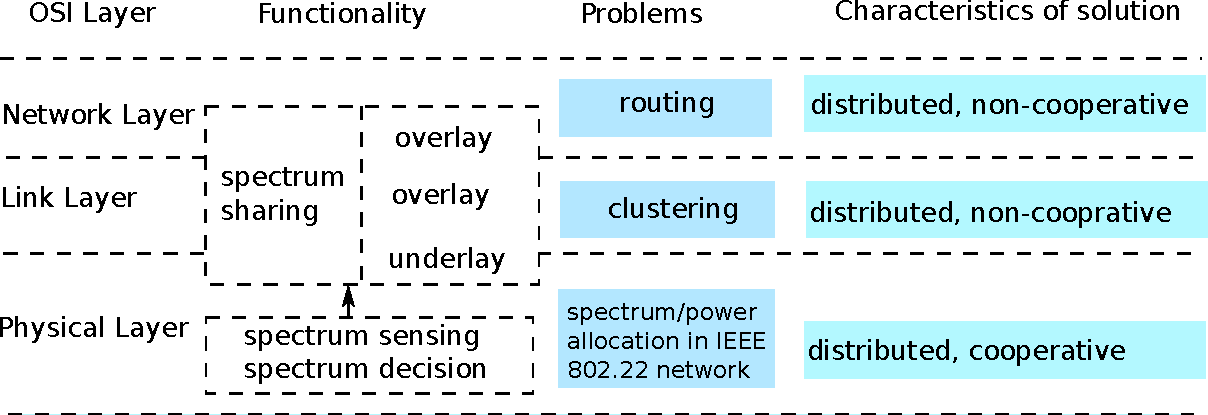
\includegraphics[width=\linewidth]{problemLocation.pdf}
  \caption{Spectrum management and the problems addressed in this thesis}
\label{problemLocation}
\end{figure}

In this thesis, some technical challenges in cognitive radio networks are shown in Figure~\ref{problemLocation}, which reside from physical layer to network work layer~\cite{osi} are addressed. 
Because of the characteristics of the problems, distributed schemes are adopted, and in order to coordinate the interaction between secondary users, game theory is used to formulate the problem and derive algorithms.

\subsection{Channel and Power Allocation in IEEE 802.22 Network}

Channel allocation facilitates CRN to improve throughput~\cite{channelAllocation_throughput_12wcnc}, or cooperatively relay~\cite{channelAllocation_relay_2010ICASSP} and so on.
This thesis emphasises on co-channel interference mitigation with distributed channel allocation . 

Mitigating co-channel interference via channel allocation has been attracting plenty of research efforts in the past ten years, from multiple channel mesh network~\cite{Hyacinth}, Ad hoc network~\cite{Babadi08, Ko_DistributedCA} up to cognitive radio network~\cite{SA_CA_TVWS_2012crowncom,qlearning_huang}. 
Channel allocation problem is converted into colouring problem thus is NP hard~\cite{Hyacinth}, thus centralized optimization fails to produce
Authors of~\cite{Babadi08, Ko_DistributedCA} propose heuristic algorithms utilizing best response based on the welfare on itself to assign channels among users.
Simulated annealing is applied to mitigate co-channel interferences in~\cite{SA_CA_TVWS_2012crowncom}.
For the same purpose, No-regret learning~\cite{qlearning_huang, hart00correlatedeq} is exploit to optimize the choice on channel.

In this thesis we cope with a special channel allocation problem where symmetric interaction doesn't exist, \ie transmission power is identical among CR users, or the propagation path loss is not symmetric. 
The asymmetry disables the heuristic distributed schemes provided in~\cite{Babadi08, Ko_DistributedCA}, and makes channel allocation problem not to fit into the congestion game model proposed in~\cite{allerton08_liu} which is the first paper to discuss channel allocation from the respective of game theory.
We innovatively formulate this problem in to a canonical congestion game by utilizing the centralized database in TV white space scenario, and derive efficient distributed channel selection strategy.
%and apply it on different cognitive radio networks.
%rethink channel allocation problem from the perspective of game theory, particularly,

\subsubsection*{Utilize TV White Space}
Unused TV spectrum is termed as TV White space by the Federal Communications Commission (FCC)~\cite{FCC_2010_sedond_memorandumm}, which is licensed to incumbent users such like digital TV, analog TV, and wireless microphone.
As to unlicensed users, detecting incumbent users is challenging because the FCC requires the unlicensed users should be able to detect the presence of signals from TV stations or wireless microphone at a received power level of -114 dBm~\cite{Technical_Challenges_TVwhit}. 
Thus FCC doesn't require the sensing ability on unlicensed users, but regulates the secondary usage of TV white space in a prudent manner, including the spectrum bands permitted to use based on their location, the transmission power, the distance away from TV service area and so on.
Every unlicensed user should register its type and geographic location to one TV database which decides which channels can be used at its places, then unlicensed user accesses the TV database to retrieve the information about available spectrum.
%This is very applicable as TV spectrum usage changes slowly, and the spectrum usage by TV stations is scheduled.
%the geographic location approach together with central database becomes more appealing in TW White Space (TVWS) utilization scenario. 
% FCC regulates portable secondary users to operate from channel 21 (512 MHz) to 51 (698 MHz), with the exception of channel 37. As to fixed secondary usage, the allowed spectrum band is from TV channel 2 (54 MHz) to TV channel 51, with TV channels 3, 4 and 37 being prohibited. Thus, the available TV spectrum is about 600 MHz wide. Compared to conventional unlicensed ISM bands in the 2.4 GHz and 5 GHz band, all together TVWS has more to offer.
Some prototype applications which only rely on the TV database are proposed in cellular network~\cite{tvwhite_lte2011, multicell_geo_dyspan11} and WiFi-like network~\cite{whitefi09} based on the FCC regulation.
  
Standardization activities are also ongoing on TVWS utilization, including 802.22~\cite{802.22} for Wireless Regional Area Networks (WRAN), IEEE 802.11af~\cite{802.11af} for WLAN, IEEE 802.15.4m~\cite{802.15.4m} for 802.15.4 wireless networks in TVWS and 802.19.1~\cite{802.19} for coexistence methods among local and Metropolitan Area Networks (MAN).
IEEE 802.22 largely complies FCC regulations on the utilization of TVWS.
System consists of base stations and customer premises equipments (or terminals for short), where each terminal is served by one base station. 
Recent standard published in Nov. 2010 suggests both sensing ability as well as database look-up to avoid affecting primary systems.
As to utilization of available TVWS, IEEE 802.22 proposes centralized channel allocation in database.
When two or more base stations co-exist on the same channel, TDMA like mechanism for WBSes is adopted.
%\cite{HoangPowerChannel2010} proposes a distributed solution for power control and channel assignment in both down-link and up-link communication in a WRAN, but the investigated secondary network is composed with only one base station and multiple terminals.

Scientific research on utilization of TVWS goes on in parallel with the regulatory agency.
Spectrum sharing in TVWS is formulated as optimization problem, where the guarantee that TV receivers should not be affected by the cumulative interferences form TVBD is one constraint, and the signal interference (noise) ratio becomes the other.
The objective can be maximizing TVBD's downlink transmission power~\cite{multipleIntf_pimrc11}, uplink transmission power~\cite{uplink_power_tvws13}, or best geographic distribution of TVBDs~\cite{withinTVcoverage_PIMRC13}.

\cite{game_CA_association_ICDCS12,SA_CA_TVWS_2012crowncom, 802.22co-existence09, 802.22game_08globecom,self-coexistenceWRAN2010infocom} emphasise on interference mitigation among TVBDs via spectrum allocation.
Vehicular networks operating with TVWS assisted by TV database and cooperative sensing is discussed in~\cite{tvws_vtc13}.
Work~\cite{increaseTVWS12} steps further from the database paradigm and makes efforts to utilize the 'grey space', where TVDB is allowed to operate even within the TV service area.

This thesis addresses following two problems,
\begin{itemize}
\item Decide the maximal downlink transmission power.
Both FCC regulation and 802.22 standard try to make TVBD transparent to incumbent users, but as long as TV system is not affected, i.e. certain quality of service is fulfilled, the strict restriction on unlicensed users can be relaxed so that more TVWS can be provided~\cite{multipleIntf_pimrc11}. 
Abiding by the operation paradigm using data base, we investigate the maximal downlink transmission power for TVBDs by solving optimization problem where the cumulative interference on TV receivers is under a threshold.

\item Distributed spectrum allocation scheme for TVBDs.
According to 802.22 regulation, spectrum allocation is done centrally in TV database, this is not realistic when TVBDs belong to different economic interest groups, thus a distributed solution is needed.
We propose efficient distributed scheme to allocate the TV channels in order to improve the quality of service of TVBDs.
The major difference between our scheme and other spectrum allocation lies in that the downlink transmission power on different channel is different.
We formulate this problem into a canonical congestion game, and derive the distributed algorithm from the best response behaviour of the player in the game. 
\end{itemize}



\subsection{Robust Clustering in Ad Hoc Cognitive Radio Network}
Clustering is an important paving stone for the practical utilization of the unused portions of the licensed spectrum.
Clustering secondary users based on geographical proximity and other relevant properties together produces following benefits.
Firstly, it is more efficient to solve common control channel (CCC) problem with cluster structure.
Dedicated CCC which is allocated to all nodes for the purpose of control information exchange is regarded to be under utilization.
Whereas, cluster based approaches group CR nodes into clusters based on their similarity of available unlicensed channels, so that the common channels within each cluster are used to carry the control messages~\cite{Lazos09}.
%whereas communication rendezvous, \ie the process to establish control channel between two CR users before they can communicate is proposed to be a economic solution.
%Within one cluster which is composed with CR nodes with similar available unlicensed channels, communication rendezvous can be accomplished within in shorter time~\cite{CommunicationRendezvous_ToN13}.
Secondly, cluster structure facilitates cooperative sensing and increases the sensing reliability~\cite{Sun07_clustering_spectrum_secsing}.
Thirdly, cluster structure supports coordinated channel switching and simplifies routing in ad-hoc cognitive radio networks~\cite{cluster_routing_2013ICC}.


There are three aspects need consideration when design a new clustering scheme.
\begin{itemize}
\item Abundance of control channels within cluster should be achieved.
A large number of control channels within cluster means high robustness.
When the current control channel gets occupied by primary user, cluster members can migrate to a new one and the cluster is maintained.
Besides, more control channels makes multiple concurrent transmission within cluster possible.
In this thesis, a distributed clustering algorithm which is especially designed to support robustness under active primary users is proposed.
Related works~\cite{Zhao07,Affinity_clustering_09icccn,Consensus_based_clustering12,clustering_globecom11} fail to pay attention to this aspect.

\item New scheme should be light weighted so that re-clustering can be quickly conducted when previous cluster is destroyed by primary user's activity.
When all the common channels are occupied by primary users, cluster head selection and following procedure is conducted by the cluster members autonomously.
\cite{LIU_TMC11_2} targets large number of control channels within cluster, but it intriguers high complexity.


\item Efficient channel allocation scheme within and among clusters is needed, so that communication rendezvous between two clusters is quick. 
Communication rendezvous means the process to establish control channel between two clusters before they can communicate .
\cite{LIU_TMC11_2} proposes channel allocation in round robin manner, but it causes long time on communication rendezvous.
\end{itemize}

These requirements will be fulfilled by the scheme proposed in this thesis.




%\section{Spectrum Aware Virtual Coordinates in CRN}
\subsection{Geographic Routing in CRN with Spectrum Aware Virtual Coordinate}
We propose a routing paradigm in CRN.
Geographic routing is applied in the CRN network which is assigned with spectrum aware virtual coordinates.
The dynamic availability of spectrum leads to prevalent topology changes, which makes spectrum aware routing difficult but essential.
Routing schemes are proposed in~\cite{Abbagnale_Gymkhana10, caodv-10wd, segment-crowncom08} for CRN where primary users change their operating parameters infrequently.
Highly dynamic primary users impose great challenge on routing, as is discussed in~\cite{Routing-crn-INFOCOM11}, where the statistics of primary users' activity is utilized in routing decision.
A class of packet forwarding strategies for dynamic spectrum CRN is proposed in~\cite{routing-crn-icc11, routing-crn-jsac12}.
Whenever a secondary user needs to forward a packet, it chooses channel and hop jointly based on channel's statistical characteristics observed beforehand.
Forwarding decision is made for each single packet, which requires complex computations, large amount of control overhead, and customized media access control mechanisms.
The solution provided by Chowdhury et al.\cite{search_geo_routing_chowdhury} improves geographic routing in multiple channel CRN by introducing circumventing mechanism, \ie when the next hop chosen based on geographic routing metric (\eg Euclidean distance) is affected by primary user, the routing packet chooses a neighbour of that node free from primary user's affection so as to avoid the primary user affected area.
Such routing is conducted on all channels, afterwards a path merge process is undertaken and one path with alternating channel is finally formed with consideration of end to end delay.

As the decision of the next hop is largely decided by the channel availability on the time point of decision, the node chosen as next hop may not be able to work after a short while due to primary user's reappearance.
Thus, this scheme works well when the primary user's activity is infrequent, but when it goes tense, the frequent invalidity of nodes due to lack of available spectrum seriously deteriorates routing performance.

In this paper we propose SAViC, spectrum aware virtual coordinates for secondary users in multi-channel multi-hop CRN where secondary users are source limited.
Virtual coordinate is independent of real geographic position, but decided by certain properties of the media among nodes, for instance, link quality or hop numbers~\cite{gpsfree05infocom}.
The proposed virtual coordinate depicts the availability of licensed spectrum influenced by primary users, on top of which geographic routing decides the next hop with Euclidean distance metric, and unconsciously detours the primary affecting area, or cuts through the area with better access opportunity.
This routing paradigm imposes little computation and communication cost on secondary users after assigning virtual coordinate, besides, it doesn't need real geographic location which is employed in ~\cite{search_geo_routing_chowdhury, routing-crn-jsac12}.

This scheme is composed with two steps,
\begin{itemize}
\item Design virtual coordinates so that virtual coordinates of any two secondary users reflect both geographic distance and opportunistic spectrum availability between them.
We design them based on statistics of primary user’s ON/OFF states which are obtained from local spectrum sensing.

\item After deciding on the next hop, we adopt a lightweight heuristic method to decide which channel to transmit packet when multiple licensed channels exist in the network.


\end{itemize}

To summarize, as the Euclidean distance between two secondary users based on spectrum aware virtual coordinate reflects the availability of unlicensed channel in between from the angel of historical statistics, virtual coordinate contributes a large part to deciding on the on the next hop. 



